\section{Discrepancies between results}
\label{sec:discrepancies}
Some of the results found throw simulations are not consistent with the claims in the article \cite{self-org}. There is also some problems with is not at all addressed.

\subsection{Clogging in narrow places}
The article \cite{self-org} claims that social force models are able to reproduce the clogging phenomena which arises when a large number of pedestrians try to pass a narrow passage. This phenomena is also know as the "faster is slower phenomena". Throw our simulation this phenomena has not occurred.



\subsection{Pedestrians overlapping and walking throw walls}
A problem we encountered during the simulation was pedestrians walking throw walls and/or pedestrians overlapping. Both these scenarios are illustrated in figure \ref{fig:problemSenario}. This could be caused by the size of the time step see section \ref{constants}, but the time step can not always correct this problem.

A person can have a resulting force which point towards the wall even as the distance to the wall approaches zero. This problem arise when pedestrians are moving fast and are unable to stop in time and occurs because the model do not take into account how fast pedestrians are approaching walls or other pedestrians.

In other words, a pedestrian running towards a wall will decelerate at the same rate as a person walking towards the wall. One could argue that this is unrealistic behaviour because, the person running should start decelerating sooner than the person walking. A person which has a force towards the wall which exceed the force he feels from the wall, then he will always go throw the wall. This phenomena is off course not dependent on the time step, since even with a infinity small time step this could occur. One way of elimination this problem is by making the force a pedestrian feel depend not only on the distance to the obstacle but also depend on the current speed towards this obstacle. Such a feature has been documented to improve the predictions of the model\cite{ABconstant}.
\begin{figure}
\centering
\subfloat[Overlapping occurs when speeds get to high in this case $2.50m/s$ which prevents pedestrians from stopping in time.]{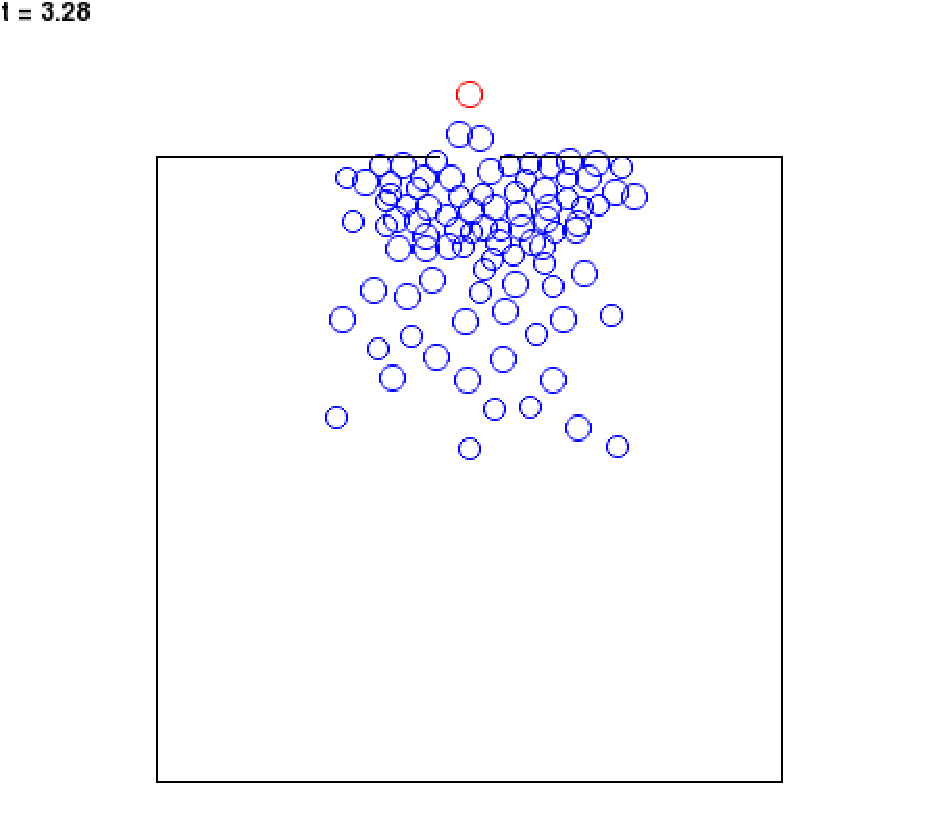
\includegraphics[scale=0.5]{Figures/squareRoomOverlapping}}
\subfloat[A single pedestrian escapes throw the wall due to a initial speed of $3.50m/s$]{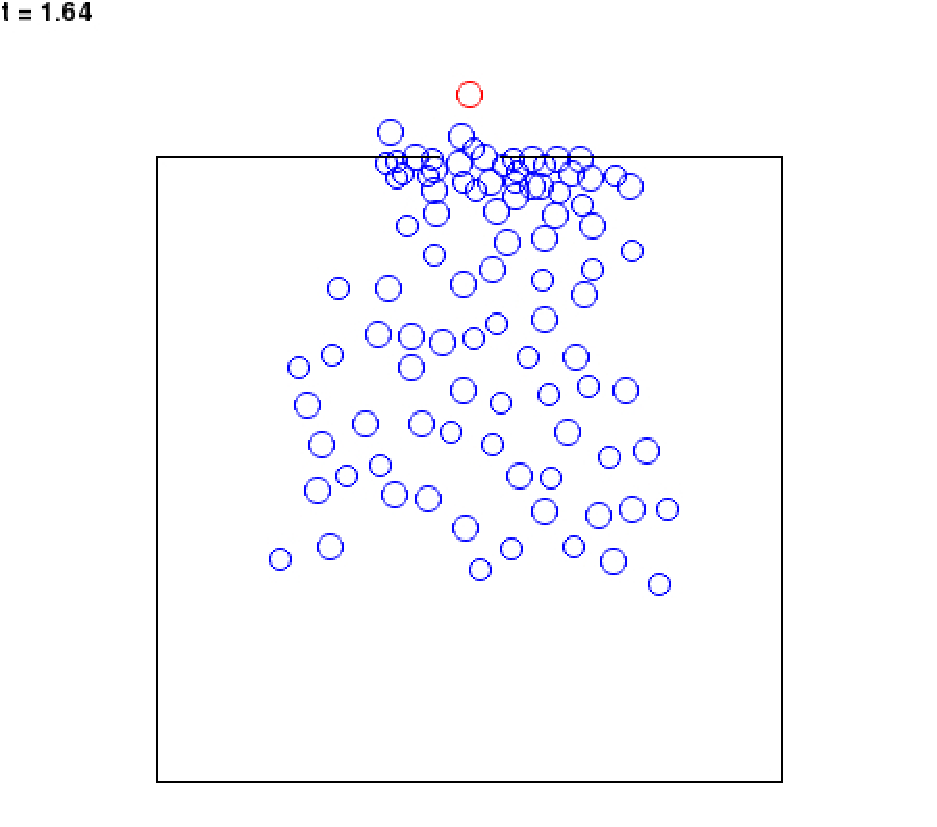
\includegraphics[scale=0.5]{Figures/squareRoomThrowWall}}
\caption{These pictures was produced with the following values: $A=2.2$, $B=0.2$, $U=2.0$, Pedestrian number=$100$, $\lambda=0.1$, $v^{max}_0=1.3 \cdot v_0$, $\tau = 1.0$, $\triangle t = 0.01$, only the starting velocity was changed}
\label{fig:problemSenario}
\end{figure}
\subsection{Faster-is-slower effect}
The article \cite{self-org} claims that social force models are models which are capable of representing the faster-is-slower effect. In our simulations people leave the room faster and faster as we increase their max speed. The article 

\subsection{Tangential forces}
Here we discuss the idea of improving the model by improving tangential forces, that is, the force parallel to the surface of an object.
The tangential forces can be used as collision avoidance, so that agents steer around obstacles or other agents \cite{tang}.
This would be relevant when simulating an environment where, e. g., and is standing in the middle of a symmetrical room and the agent's waypoint
is behind a big square pillar, with equal distance either way around, the agent would get stuck in front of the pillar without the tangential forces,
since the forces acting on the agent's motivation is cancelling each other out. 
In our case where two groups of agents are crossing each other in a corridor, the tangential force would make the agents to into account
the position of the agents in front of them and steer around them.
The tangential forces can also improve the model so it can simulate agents escaping a smoke filled room where we determine the visibility.
In this case of simulation the agents would walk randomly around untill they find a wall, and follow the wall around due to the tangential force.
This would be a way of implementing way finding to the model.

Friction between agents would also be possible to add to the model, since the tangential forces from other agents would make it
harder for agents to walk through a crowd. \cite{self-org} mention that friction is causing clogging in front of exits, since the people
get stuck in each other. In our simulation the agents are not clogging as heavily as \cite{self-org} mention it can be.
The time it take for the agent to leave a room in unrealistic low, and we think that implementing the friction by tangential forces
would make the simulation time more realistic.
